\documentclass[tikz,border=5pt]{standalone}
\usepackage[UTF8]{ctex}\usepackage{amsmath,amssymb}
\usetikzlibrary{arrows.meta,calc}
\definecolor{ink}{HTML}{243447}\definecolor{blue}{HTML}{2765A2}
\definecolor{green}{HTML}{3F7D5B}\definecolor{red}{HTML}{B74739}
\tikzset{body/.style={draw=ink,thick},vec/.style={draw=blue,thick,-{Latex}},guide/.style={gray!65,dashed},dim/.style={ink,{Latex}-{Latex}},line cap=round,line join=round}
\begin{document}
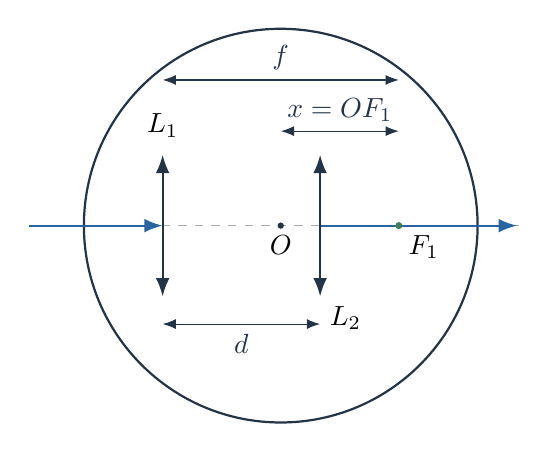
\begin{tikzpicture}
 \draw[body](0,0)circle(2.5);
 \draw[guide](-3.2,0)--(3.1,0);
 \draw[vec](-3.2,0)--(-1.5,0);\draw[vec](.5,0)--(3,0);
 \draw[body,{Latex}-{Latex}](-1.5,-.9)--(-1.5,.9);
 \draw[body,{Latex}-{Latex}](.5,-.9)--(.5,.9);
 \node[above]at(-1.5,1){$L_1$};\node[below right]at(.5,-.9){$L_2$};
 \fill[ink](0,0)circle(.04);\node[below]at(0,0){$O$};
 \fill[green](1.5,0)circle(.045);\node[below right]at(1.5,0){$F_1$};
 \draw[dim](-1.5,-1.25)--(.5,-1.25)node[midway,below]{$d$};
 \draw[dim](-1.5,1.85)--(1.5,1.85)node[midway,above]{$f$};
 \draw[dim](0,1.2)--(1.5,1.2)node[midway,above]{$x=OF_1$};
\end{tikzpicture}
\begin{tikzpicture}
 \pgfmathsetmacro{\ang}{12}
 \pgfmathsetmacro{\yin}{1.5*tan(\ang)}
 \pgfmathsetmacro{\slope}{-\ang*pi/180-\yin/3}
 \pgfmathsetmacro{\yout}{\yin+2*\slope}
 \draw[guide](-3.1,0)--(3.4,0);
 \node[above right,text=gray]at(2.5,.05){固定入射线};
 \begin{scope}[rotate=\ang]
 \draw[green,thick](-2.7,0)--(2.5,0)node[above right]{旋转光轴};
 \draw[body,{Latex}-{Latex}](-1.5,-.86)--(-1.5,.86);
 \draw[body,{Latex}-{Latex}](.5,-.86)--(.5,.86);
 \coordinate(Pone)at(-1.5,\yin);
 \coordinate(Ptwo)at(.5,\yout);
 \draw[vec](Pone)--(Ptwo);
 \node[below]at(-1.5,-.95){$L_1$};
 \node[above]at(.5,.95){$L_2$};
 \draw[guide](-2.05,0)--(-1.5,0);
 \draw[guide](-2.05,\yin)--(Pone);
 \draw[dim](-2.05,0)--(-2.05,\yin)node[midway,left]{$y_1$};
 \draw[guide](.5,0)--(1.28,0);
 \draw[guide](Ptwo)--(1.28,\yout);
 \draw[dim](1.28,\yout)--(1.28,0)node[midway,right]{$y_2<0$};
 \end{scope}
 \draw[vec](-3.1,0)--(Pone);
 \draw[vec](Ptwo)--($(Ptwo)+(2.6,0)$);
 \fill[ink](0,0)circle(.04);\node[above left]at(0,0){$O$};
 \draw[blue,-{Latex}](.85,0)arc[start angle=0,end angle=12,radius=.85];
 \node[blue,above]at(.85,.24){$\theta$};
\end{tikzpicture}
\begin{tikzpicture}
 \pgfmathsetmacro{\ang}{10}
 \pgfmathsetmacro{\yin}{1.5*tan(\ang)}
 \pgfmathsetmacro{\slope}{-\ang*pi/180-\yin/3}
 \pgfmathsetmacro{\yout}{\yin+2*\slope}
 \pgfmathsetmacro{\ystar}{\yin+3*\slope}
 \draw[guide](-3.1,0)--(3.1,0);
 \begin{scope}[rotate=\ang]
 \draw[green,thick](-2.6,0)--(2.4,0);
 \draw[body,{Latex}-{Latex}](-1.5,-.8)--(-1.5,.8);
 \draw[body,{Latex}-{Latex}](.5,-.8)--(.5,.8);
 \coordinate(Pone)at(-1.5,\yin);
 \coordinate(Ptwo)at(.5,\yout);
 \draw[vec](Pone)--(Ptwo);
 \draw[red,dashed,thick](Ptwo)--(1.5,\ystar);
 \fill[green](1.5,0)circle(.04);\node[above]at(1.5,0){$F_1$};
 \fill[red](1.5,\ystar)circle(.04);\node[below]at(1.5,\ystar){$F_*$};
 \draw[guide](1.5,0)--(2.05,0)(1.5,\ystar)--(2.05,\ystar);
 \draw[dim](2.05,\ystar)--(2.05,0)node[midway,right]{$|y_*|$};
 \node[below]at(-1.5,-.9){$L_1$};\node[below]at(.5,-.9){$L_2$};
 \end{scope}
 \draw[vec](-3.1,0)--(Pone);
 \draw[vec](Ptwo)--($(Ptwo)+(2.7,0)$)node[below right]{平行出射};
 \fill[ink](0,0)circle(.035);\node[above left]at(0,0){$O$};
\end{tikzpicture}
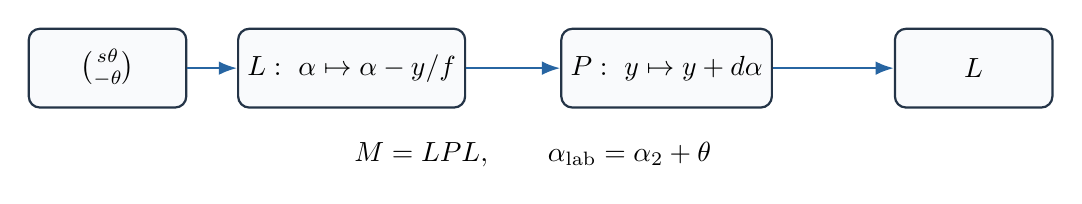
\begin{tikzpicture}
 \node[body,rounded corners,fill=blue!3,minimum width=2cm,minimum height=1cm](A)at(0,0){$\binom{s\theta}{-\theta}$};
 \node[body,rounded corners,fill=blue!3,minimum width=2cm,minimum height=1cm](B)at(3.1,0){$L:\ \alpha\mapsto\alpha-y/f$};
 \node[body,rounded corners,fill=blue!3,minimum width=2cm,minimum height=1cm](C)at(7.1,0){$P:\ y\mapsto y+d\alpha$};
 \node[body,rounded corners,fill=blue!3,minimum width=2cm,minimum height=1cm](D)at(11,0){$L$};
 \draw[vec](A)--(B);\draw[vec](B)--(C);\draw[vec](C)--(D);
 \node at(5.4,-1.1){$M=LPL,\qquad \alpha_{\rm lab}=\alpha_2+\theta$};
\end{tikzpicture}
\end{document}
